% tikzposter.tex, version 2.0
% Original template created by Elena Botoeva [botoeva@inf.unibz.it], June 2012
% 
% This file is distributed under the Creative Commons Attribution-NonCommercial 2.0
% Generic (CC BY-NC 2.0) license
% http://creativecommons.org/licenses/by-nc/2.0/ 


\documentclass{a0poster}

\usepackage{fancytikzposter}
\usetikzlibrary{arrows}
\usepackage{calligra}
\usepackage{FMcommands}

%%%%% --------- Change here if you want ---------- %%%%%
%% margin for the geometry package, must be changed before using the geometry package
%% default value is 4cm
\setmargin{1.5}

%% the space between the blocks
%% default value is 2cm
\setblockspacing{1}

%% the height of the title stripe in block nodes, decrease it to save space
%% default value is 3cm
\setblocktitleheight{1cm}

%% the number of columns in the poster, possible values 2,3
%% default value is 2
\setcolumnnumber{2}

%% the space between two or more groups of authors from different institutions
%% used in \maketitle
% \setinstituteshift{10}

%% which template to use
%% N1 simple, standard look, with a colored background and gray boxes
%% N2 board with nodes
%% N3 another standard look
%% N4 envelope-like look
%% N5 with a wave-like head, original idea taken from
%%%% http://fc09.deviantart.net/fs71/f/2010/322/1/1/scientific_poster_by_nabuy-d333ria.jpg
\usetemplate{2}

%% components of the templates
%% (the maximal possible numbers are mentioned as the parameters)
% \usecolortemplate{2}            % max 4
% \usebackgroundtemplate{2}       % max 5
% \usetitletemplate{1}            % max 2
% \useblocknodetemplate{5}        % max 5
% \useplainnodetemplate{4}        % max 4
% \useinnernodetemplate{2}        % max 2


%% the height of the head drawing on top 
%% applicable to templates N3, 4 and 5
% \setheaddrawingheight{11}


%% change the basic colors
\definecolor{fbw1}{HTML}{22BCB9} 
\definecolor{fbw2}{HTML}{2272BC} 
\definecolor{fbw3}{HTML}{22A3A0} 
\definecolor{ugent1}{HTML}{0A1E60} 
\definecolor{ugent2}{HTML}{FFB300}
\definecolor{ugent3}{HTML}{0A4960}
\definecolor{myGray}{HTML}{CCCCCC} 
%\definecolor{myblue}{HTML}{008888} 
%\setfirstcolor{myblue}% default 116699
%\setsecondcolor{gray!80!}% default CCCCCC
%\setthirdcolor{red!80!black}% default 991111

%% change the more specific colors
% \setbackgroundlightcolor{colorone!70!}
% \setbackgrounddarkcolor{colorone!70!black}
\setbackgroundlightcolor{ugent1}   %ugent1
\setbackgrounddarkcolor{fbw3}    %fbw1

\settitletextcolor{white} 
% \settitletextcolor{textcolor}
% \settitlefillcolor{white}
% \settitledrawcolor{colortwo}
% \setblocktextcolor{textcolor}
% \setblockfillcolor{white}
% \setblocktitletextcolor{colorone}
% \setblocktitlefillcolor{colortwo} %the color of the border
% \setplainblocktextcolor{textcolor}

\setplainblockfillcolor{colorthree!15!}
% \setplainblockfillcolor{yellow!20!}

% \setplainblocktitletextcolor{textcolor}
% \setplainblocktitlefillcolor{colorthree!60!}
% \setinnerblocktextcolor{textcolor}
%\setinnerblockfillcolor{white}
% \setinnerblocktitletextcolor{white}
% \setinnerblocktitlefillcolor{colorthree}

%%%- FREE TEXT BLOCK    -%%%
%% the content of the block
% #1 - where
% #2 - title
% #3 - text
% #4 - width
\newcommand{\mydrawnode}[4]{
\draw let \p1=($(#4)-(2.3,0)$) in 
    node[draw,anchor=north west, color=blocktitlefillcolor, 
%     fill=backgroundlightcolor!70!, text=blocktextcolor, frametwo, rectangle, 
    fill=plainblockfillcolor, text=blocktextcolor, frametwo, %
    rectangle, rounded corners=10]% 
    (box) at #1 {
    \begin{minipage}{\x1}
%         \vspace{0.2cm}
%         {\footnotesize\bfseries\textcolor{blocktitletextcolor}{#2}}\\
        \color{blocktextcolor}
        #3
    \end{minipage}};
}
\newcommand{\myblocknode}[4][(currenty)]{%
  %% width = (#2) - 0.3
  %% 
  %% 
  \coordinate (width) at ($(#2,0) - (0.3,0)$);   
  
  \mydrawnode{#1}{#3}{#4}{width}
}

%%% size of the document and the margins
%% A0594 � 841
\usepackage[margin=\margin cm,
%   paperwidth=59.2cm,paperheight=83.9cm]{geometry}
  paperwidth=83.9cm,paperheight=118.5cm]{geometry}
%     paperwidth=118.9cm,paperheight=83.9cm]{geometry}
% \usepackage[margin=\margin cm, paperwidth=84.1cm,
%     paperheight=118.9cm]{geometry}
%% B1
% \usepackage[margin=\margin cm, paperwidth=70cm, paperheight=100cm]{geometry}
%% A4
% \usepackage[margin=\margin mm, paperwidth=210mm, paperheight=297mm]{geometry}



%% changing the fonts
\usepackage{cmbright}
%\usepackage[default]{cantarell}
%\usepackage{avant}
%\usepackage[math]{iwona}
\usepackage[math]{kurier}
\usepackage[T1]{fontenc}
\usepackage{multirow}


%% add your packages here
% \usepackage{hyperref}
\usepackage[bookmarks,colorlinks,breaklinks,unicode,%
pdftitle={TiKZ Resume},%
pdfauthor={Federico Mattiello}]{hyperref}
\hypersetup{linkcolor=myRoyalBlue1,citecolor=myRoyalBlue1,%
  filecolor=myRoyalBlue1,urlcolor=fbw1,%black!60!,%
  pdfstartview={FitV},    % Fit, FitH, FitV, FitBH, FitBV, XYZ null null 1.00
  pdfpagelayout={OneColumn}}    % OneColumn, SinglePage, TwoPageLeft }
\usepackage{graphicx}
\graphicspath{{figures/}}
\usepackage{array} 
\usepackage[singlespacing]{setspace}        % to set the lineskip



\title{% 
%   \begin{tabular}{llr}
%     \multirow{2}{*}{Federico \ Mattiello} & \hspace{.6\linewidth} & 
%     \multirow{3}{*}{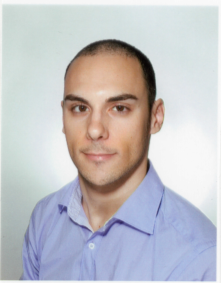
\includegraphics[height=2in]{IDphoto.pdf}}\\
%     {\footnotesize
%     \textcolor{gray!60!}{Phone: {+32} 483 60 21 91}} & & \\
%     %\hspace*{.2\linewidth}
%     {\footnotesize
%     \textcolor{gray!30!}{Email: \url{federico.mattiello@gmail.com}}}
%     & & 
%   \end{tabular}%\vspace*{2em}
  \begin{minipage}{1.5\linewidth}
    Federico  Mattiello\\
    {\footnotesize
      \textcolor{gray!20!}{Phone: }\textcolor{gray!60!}{{+32} 483 60 21 91}
      \hspace{1em} 
      \textcolor{gray!30!}{Email: \url{federico.mattiello@gmail.com}}}
  \end{minipage}\hspace*{.2\linewidth}  % & %
  \begin{minipage}{.5\linewidth}
%   \vspace*{2.1em}
  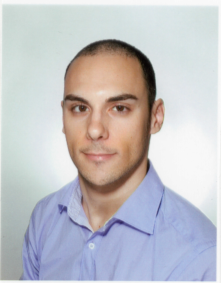
\includegraphics[height=1.8in,trim=10 15 5 15,clip]{IDphoto.pdf}
  \end{minipage}
}
\author{ 
% \hspace*{\linewidth}
% {\footnotesize
% \textcolor{gray!60!}{Phone: {+32} 483 60 21 91} \hspace*{.2\linewidth}
% \textcolor{gray!30!}{Email: \url{federico.mattiello@gmail.com}}}
% \vspace*{.5em}
} 
 


%%%-----------------------------%%%
%%%     BEGIN OF THE DOCUMENT   %%%
%%%-----------------------------%%%


\begin{document}

%%%%% ---------- the background picture ---------- %%%%%
%% to change it modify the macro \BackgroundPicture
\ClearShipoutPicture
\AddToShipoutPicture{\BackgroundPicture}

\noindent % to have the picture right in the center
\begin{tikzpicture}
\initializesizeandshifts
% \setxshift{15}
% \setyshift{2}

%% the title block, #1 - shift, the default value is (0,0), #2 - width, #3 - scale
%% the alias of the title block is `title', so we can refer to its boundaries later
\titleblock{15}{2.5} 
 
%% a logo can be added to the title block
%% #1 - anchor relative to the title block, #2 - shift, #3 - width, #3 - file name
  % % \addlogo[south west]{(-2,0)}{8cm}{Ugent_bigLogo.png}
%     \addlogo[north west]{(-21,0)}{13cm}{UGentBigLogoTranspW.png}
%     \addlogo[north east]{ (21,-1)}{14cm}{Biostat.png}
%   % \ifthenelse{\equal{\template}{2}}{ 
%   %   \addlogo[south west]{(2,0)}{6cm}{unibz_b.png}
%   % }{
%   %   \addlogo[south west]{(2,0)}{6cm}{unibz_w.png}
%   % }


  %% a block node, with the specified position (optional), title and the
  % content
  %% #1 - where (optional), #2 - title, #3 - text
  %%%%%%%%%% ------------------------------------------ %%%%%%%%%%
%     \blocknode%
  %%%- NEW BLOCK
  \blocknodew[($(currenty)+(0,5)$)]{40}%
  {\Huge Current}%
  {\LARGE
  \begin{description}  
  \item[\textbfcol{myRoyalBlue2}{\LARGE 04/2012 -- today:}] \ \ 
    \textbf{Researcher}/Ph.D. student at the Department of ``Mathematical
    Modelling, Statistics and Bioinformatic'', Ghent University, Gent.
  \end{description}
  \textbf{Topics:} \ statistical data integration in early-stage drug
    development, differential abundance in gut microbiome experiments.
  }
  
  %%%- NEW BLOCK
  \blocknodew[($(currenty)-(0,0)$)]{40}%
  {\Huge Education}%
  {\LARGE
    \begin{description}  
    \item[\textbfcol{myRoyalBlue2}{\LARGE 10/2010 -- 02/02/2015:}] \ \ 
      \textbf{Ph.D. degree} \\ 
      at Department of ``Statistical Sciences'', University of Bologna,
      Bologna.
      Title of the thesis: {\em ``Permutation-Based Stochastic Ordering Using
      Pairwise Comparisons''}
    \item[\textbfcol{myRoyalBlue2}{\LARGE 10/2008 -- 07/2010:}] \ \ 
      Master's degree \\
      in ``Statistics and Informatics'', University of Padova, Padova.
    \item[\textbfcol{myRoyalBlue2}{\LARGE 10/2004 -- 03/2008:}] \ \ 
      Bachelor's Degree \\
      in ``Statistics and Information Technologies'', University of Padova, Padova.
    \item[\textbfcol{myRoyalBlue2}{\LARGE 09/1999 -- 07/2004:}] \ \ 
      High School Diploma, \\
      Industrial-Technical Certificate, specialisation in Computer Science, 
      I.T.I.S., Este.%\footnotemark
    \end{description}
    \setcounter{footnote}{0}%
}


%% a callout node
%% #1 - rotate angle (optional), #2 - from, #3 - where, #4 - width, #5 - text
%%%%%%%%%% ------------------------------------------ %%%%%%%%%%
%     \calloutnode {($(box.center)+(-2,-8)$)}
%     {($(box.center)+(10,-1)$)}
%     {19cm}
%     {\small
%         Macro for creating a block node:
%         \begin{itemize}
%         \item[] \textbackslash blocknode\{Block Title\}\{Block Content\}
%         \end{itemize}
%         Macro \textbackslash blocknode has three parameters. The first one is
%         optional and it is the position of the block. The first block will be
%         automatically placed to (\$(firstrow)-(xshift)-(yshift)\$), which is the
%         left corner below the title block. In most of the templates, (firstrow) is
%         set to (title.south), where \emph{title} is the alias for the title
%         block. Each subsequent block is automatically placed to
%         [(\$(box.south)-(yshift)\$)], i.e., below the previous block aliased
%         \emph{box}.  You can also use an explicit parameter, e.g., $(-10,30)$ (note
%         that (0,0) is the center of the poster). The second parameter is the title
%         of the block. Finally, the last parameter is the  actual content. 
%     }



%     \calloutnode {($(box.center)+(2,8)$)}
%     {($(box.center)+(-4,3)$)}
%     {.25\columnwidth}
%     {\small
%     \textbfcol{myRoyalBlue2}{{\Large Q}}uantitative 
%     \textbfcol{myRoyalBlue2}{{\Large S}}tructure 
%     \textbfcol{myRoyalBlue2}{{\Large T}}ranscriptional 
%     \textbfcol{myRoyalBlue2}{{\Large A}}ctivity 
%     \textbfcol{myRoyalBlue2}{{\Large R}}elationship\\
%     %
%     % \includegraphics[height=.91\textheight]{magicTriangle.png}
%     \includegraphics[height=.13\textheight]{qstarTriangle.png}
%     }




%% by default, the position of the new block node is right below the previous
%% block node, stored in (currenty)
%% box is the alias of the previous block, so we can refer to its boundaries

  %%%- NEW BLOCK
  \blocknodew[($(currenty)-(0,0)$)]{40}%
  {\huge Research Collaborations}%
  {\Large
    \begin{description}  
    \item[\textbfcol{myRoyalBlue2}{\Large IAP-StUDyS:}] \ \ 
      within the network of projects funded by the E.U. (belonging to ``Phase
      VII'' implementation) through the Belgian Science Policy Office. Topic
      I'm focusing on is developing models for \textbf{microbiome 16S sequencing
      data}.
    \item[\textbfcol{myRoyalBlue2}{\Large QSTAR:}] \ \ 
      project funded by the Flemish ``Agency for Innovation by
      Science and Technology'', and by Janssen Pharmaceutica. Main goal was to
      assess if \textbf{integration of transcriptomics data} into early-stage
      drug development could help the decision-making process
      (\url{qstar-consortium.org}).
    \end{description}
}


  %%%%%%%%%% ------------------------------------------ %%%%%%%%%%
%     \blocknodew[($(currenty)+(8,0)$)]{50}{Variable Width Block Nodes} %
%     {
%     You can also create blocks of arbitrary width
%     \begin{itemize}
%     \item[] \textbackslash blocknodew[coordinate]\{Block width\}\{Block Title\}%
%       \{Block Content\}
%     \end{itemize} 
%     % 
%     In this case it is better to specify coordinate manually if you want to have
%     blocks aligned vertically. \\
% 
%     Note that (xshift) and (yshift) are coordinates created in macro
%     \textbackslash initializesizeandshifts, and they allow to have relative
%     positioning of block nodes in an automatic fashion. If you want to define
%     your own shifts, set new values for (xshift) and (yshift) using commands
%     \textbackslash setxshift and \textbackslash setyshift.\\
% 
%     Also, it might be useful to know the y-coordinate of the south border of the
%     previous block. You can retrieve it by using the command
%     \begin{itemize}
%     \item[] \textbackslash getcurrentrow\{box\} or \textbackslash
%     getcurrentrow\{note\}
%     \end{itemize}
%     This coordinate will be stored in (currentrow), which can be used to specify
%     the location of the next block node.
%     }

  \plainnode{($(currenty)+(0,0)$)}{40}%
  {\huge Publications}%
  {\Large 
  \begin{itemize}
    \item 
      \textbf{Federico Mattiello}, \etal.\
      A Web Application for Sample Size and Power Calculation in Case-Control
      Microbiome Studies.\ Submitted in June to \emph{Bioinformatics}. 
    \item 
      \textbf{Federico Mattiello}, Olivier Thas, and Bie Verbist (2015).\
      Principal Bicorrelation Analysis: Unraveling Associations Between Three
      Data Sources.\ \emph{Journal of Biopharmaceutical Statistics}. \ 
      To appear.
    \item 
      \textbf{Federico Mattiello} (2015).\ %
      Permutation-Based Stochastic Ordering Using Pairwise Comparisons.\ 
      \emph{Ph.D. Thesis}. Doctorate in ``Statistical Methodology for The
      Scientific Research'' 
      (\href{http://amsdottorato.unibo.it/6735/1/Mattiello_Federico_tesi.pdf}{
      direct link}).
%     \item  
%       \textbf{Federico Mattiello}, Mario Bolzan and Licia Ravarotto (2012).
%       Assessing perceived food chemical risk by means of an educational 
%       project analysed with permutation tests. \emph{Quaderni di Statistica},
%       14:165-168, 2012.
      \item  
        Rosa G. Arboretti, Livio Corain, Daniele Gomiero, and \textbf{Federico
        Mattiello} Nonparametric multivariate ranking methods for global
        performance indexes. \emph{Quaderni di Statistica}, \textbf{12}:79-106,
        2010
  \end{itemize}
  }
  
  
    \setplainblockfillcolor{ugent1!80!}
%   \setplainblockfillcolor{colorthree!20!}
  \setblocktitleheight{.5cm}
  
  \plainnode[3]{($(currenty)+(0,-24)$)}%[($(currenty)+(0,10)$)]%
  {26}{}%
  {\Large
    \textcolor{black!100!}{%
    \href{https://www.linkedin.com/profile/view?id=125233914}{LinkedIn}}
    \hspace{3em}
    \textcolor{black!100!}{%
    \href{https://www.researchgate.net/profile/Federico_Mattiello}{ResearchGate}}
  }
  
  
  %%%%%%%%%%%%% NEW COLUMN %%%%%%%%%%%%%%% 
  \startsecondcolumn 

  %%%- NEW BLOCK
  \blocknodew[($(currenty)+(0,5)$)]{40}%
  {\Huge ``Hard'' Skills}% 
  {\LARGE
  \begin{description} 
    \item[\textbfcol{myRoyalBlue2}{R:}] \ \ 
      Advanced knowledge/power user.
    \item[\textbfcol{myRoyalBlue2}{Reporting:}] \ \ 
      in particular with {\bfseries R}, {\bfseries knitr} and {\bfseries
      \LaTeX}
    \item[\textbfcol{myRoyalBlue2}{Shiny$^\text{\small\textcopyright}$:}] \ 
      for developing interactive web application with
      {\bfseries R} as underlying workhorse.
    \item[\textbfcol{myRoyalBlue2}{Others:}] \ \ 
      some {C++} experience, Windows$^\text{\small\textcopyright}$ and Linux
      (limited knowledge) OSs.
  \end{description}
  }
  
  
  
  %%% NEW BLOCK
  \blocknodew[($(currenty)+(0,0)$)]{40}%
  {\Huge ``Soft'' Skills}%
  {\LARGE
    \begin{itemize}
      \item 
        I'm always \textbf{interested in learning}, looking for cultural
        and scientific stimuli. Whether you come from Taiwan (just
        an example), or you want to talk about (bio)statistics, physics,
        oriental philosophy, movies, literature etc. I'm all ears (well, I talk
        as well of course).
      \item 
        Presenting to a non-statistical audience it's fun, because I
        have to remove frills and convey the take-home message effectively.
      \item 
        I'm open-minded and collaborative when in a team, but if I see that 
        something can be done better by myself I go for it.
      \item  
        I do my best when I \textbf{face new problems} that challenge me 
        intellectually and that require reasoning and creativity.
        I'm not satisfied until the work is well done, although I can live with
        (barely) sub-optimal ones in case of narrow deadlines.
    \end{itemize}
  }
  
  
  %%% NEW BLOCK
  \blocknodew[($(currenty)+(0,0)$)]{40}%
  {\Huge Interests}%
  {\Large
    \begin{description}
      \item[\textbfcol{myRoyalBlue2}{Research:}] \ \ 
        high-dimensional data, data integration, permutation tests and
        NonParametric Combination Methodology, Probabilistic
        Index Models, regularization (sparse) methods, statistical simulation,
        statistical modelling, machine learning\ldots basically
        anything related to (bio)statistics.
      \item[\textbfcol{myRoyalBlue2}{Personal:}] \ \ 
        I like to read books related to statistics, mathematics, popular
        science (physics, mathematics, logic), psychology, oriental philosophy,
        and novels dealing with journeys and different cultures.
        I like a lot of movies but my favourite ones come from Italy,
        Japan, France, U.K., Hollywood, and Bollywood.
    \end{description}
  }
  
  
  
    %%%- NEW BLOCK
  \blocknodew[($(currenty)+(0,0)$)]{40}%
  {\Huge Languages}%
  {
    \begin{center} 
      \coloredboxw{.75\columnwidth}{colorthree!70!}{%
      \Large
      \begin{tabular}{rcccc}
        & \multicolumn{2}{c}{Understanding} & Speaking & Writing \\
        & Listening & Reading & & \\
        \hline
        \textbf{Italian}: & \multicolumn{4}{c}{Native Language} \\
        \textbf{English:} & C1\footnotemark & C1 & C1 & C1 \\
        \textbf{Dutch:} & B2 & B2 & B1 & B1 \\
        \textbf{French:} & A1 & A1 & A1 & A1 \\
        \textbf{Spanish:} & A1 & A1 & A1 & A1 \\
        \hline
      \end{tabular}
      }\setcounter{footnote}{0}
    \end{center}
    \rule{0em}{1em}
    \footnotetext{\textsuperscript{\large\textcolor{myRoyalBlue1}{a}}\ %
    \normalsize C1: Proficient User, B1-B2: Independent User, A1: Basic User}
  }
  
  
  
  %%%%%%%%%% ------------------------------------------ %%%%%%%%%%
  %%%- callout node, it refers to the PBA steps!
  %% #1 - rotate angle (optional), #2 - from, #3 - where, #4 - width, 
  %% #5 - text
%     \calloutnode {($(box.north)+(-2.5,10)$)}%
%     {($(box.north)+(12.5,20)$)}%
% %     \calloutnode {($(currentx)-(4,2.5)$)}
% %     {($(currentx)+(12,5)$)}
%     {25cm}
%     {%\small
%     }
  
  
  
  %%%%%%%%%% ------------------------------------------ %%%%%%%%%%
  
  
  
  
  
%   \blocknode%
%   \blocknodew[($(currenty)-(0,0)$)]{40}%
%   {Colored Boxes Inside Block Nodes}%
%   {There are three types of colored boxes/blocks that you can use inside block
%     nodes to highlight information. \\
%     
%     \begin{tabular}[t]{ll}
%       \begin{minipage}{0.5\linewidth}
%         \innerblock{Theorem} {Statement}
%       \end{minipage}
%       & 
%       \textbackslash innerblock\{Theorem\}\{Statement\}\\
% 
%       \begin{minipage}{0.5\linewidth}
%         \innerblockplain[colorone!80!]{Text}
%       \end{minipage}
%       &
%       \textbackslash innerblockplain[colorone!80!]\{Text\}\\ 
% 
%       \begin{minipage}{0.5\linewidth}
%         \coloredbox{colorthree!50!}{Text}
%       \end{minipage}
%       &
%       \textbackslash coloredbox\{colorthree!50!\}\{Text\}
%     \end{tabular}
% 
%   }



  %% to place the next node centered vertically in the second column, we can
  %% obtain the y-coordinate of the previous node using macro
  %% \getcurrentrow{note}, where note is the alias of the callout node, and
  %% then specify the coordinate of the next node using coordinate 
  %% (currentrow)
  \getcurrentrow{note}



  \getcurrentrow{note}
  \coordinate (currenty) at ($(currentrow)+(xshift)-(yshift)$);




  %%%%%%%%%%%%% NEW COLUMN %%%%%%%%%%%%%%% 
  %% (if column number is 3)
%   \startthirdcolumn
  
  
  %%%%%%%%%% ------------------------------------------ %%%%%%%%%%
  % \blocknode%
%     \blocknodew[($(currenty)+(3,0)$)]{40}%
%     {Simulation Study}%
%     {
%     \begin{tabular}{%
%         p{.34\columnwidth}%
%         p{.31\columnwidth}%
%         p{.35\columnwidth}}
%     \coloredboxw{.34\columnwidth}{colorthree!50!}{\small\flushleft
%     $10$ FFs ($1^\text{st}$ type) are built to create this 
%     dependence:\vspace{1em}
%     tntnnnttn
%     } & %
% %     \hspace*{.005\columnwidth}
%     %
%     \coloredboxw{.315\columnwidth}{colorthree!50!}{\small\flushleft
%     $10$ FFs ($2^\text{nd}$ type) are built to create this dependence:%
%     ntntntnt
%     } & %
%     %
%     \coloredboxw{.355\columnwidth}{colorthree!50!}{\small\flushleft
%     $10$ FFs ($3^\text{rd}$ type) are built to create this dependence:%
%     \vspace{1em}
%     nntnnt
%     } %
%     \end{tabular}\vspace*{-1.8em}
%     
%     }
  
  
  
%     \blocknodew[($(currenty)+(0,0)$)]{40}%
%     {Simulation Results}%
%     {
%     text text text text 
%     }
  
  
  
%     \setplainblockfillcolor{colorthree!20!}
%     \plainnode{($(currenty)+(0,0)$)}%[($(currenty)+(0,10)$)]%
%     {40}{Conclusions}%
%     {
%     This is my final conclusion.
%     }
  
  
  
%   \setplainblockfillcolor{ugent1!80!}
% %   \setplainblockfillcolor{colorthree!20!}
%   \setblocktitleheight{.5cm}
%   
%   \plainnode[3]{($(currenty)+(0,2)$)}%[($(currenty)+(0,10)$)]%
%   {26}{}%
%   {\Large
%     \textcolor{black!100!}{%
%     \href{https://www.linkedin.com/profile/view?id=125233914}{LinkedIn}}
%     \hspace{3em}
%     \textcolor{black!100!}{%
%     \href{https://www.researchgate.net/profile/Federico_Mattiello}{ResearchGate}}
%   }
  
  %%%%%%%%%% ------------------------------------------ %%%%%%%%%%
  %% a plain node
  %% #1 - rotate angle (optional), #2 - where, #3 - width, #4 - title,
  %% #5 - text
  %%%%%%%%%% ------------------------------------------ %%%%%%%%%%
%     \plainnode[3]{($(currenty)+(0,-8.5)$)}%[($(currenty)+(0,10)$)]%
%     {31}{References}%
%     {\small
%         \begin{itemize}
%             \item 
%                 Witten D.M., Tibshirani R.J. and Hastie T. (2009).\ %
%                 A penalized matrix decomposition, with applications to sparse
%                 principal components and canonical correlation analysis.\ 
%                 \emph{Biostatistics}, $(\mathbf{10})$, $515 \! - \! 534$
%             \item 
%                 Witten D.M. and Tibshirani R.J. (2009).\ %
%                 Extensions of Sparse Canonical Correlation Analysis with
%                 Applications to Genomic Data.\ 
%                 \emph{Statistical Applications in Genetics and Molecular
%                 Biology}, Volume $\mathbf 8$, Issue $\mathbf 1$ 
%                 Article $\mathbf{28}$
%         \end{itemize}
%     }
  
  
  
  
  


%   \myblocknode[($(currenty)+(0,-8.5)$)]%
%   {26}{}%
%   {\Large  
%     \textcolor{black!100!}{%
%     \href{https://www.linkedin.com/profile/view?id=125233914}{LinkedIn}}
%     \hspace{3em}
%     \textcolor{black!100!}{%
%     \href{https://www.researchgate.net/profile/Federico_Mattiello}{ResearchGate}}
%   }

  
%   \myblocknode[($(currenty)+(3,-28)$)]{16}%
%   {}%
%   {
%     \textcolor{black!70!}{%
%     \href{https://www.linkedin.com/profile/view?id=125233914}{LinkedIn}}\\
%     \textcolor{black!70!}{%
%     \href{https://www.researchgate.net/profile/Federico_Mattiello}{ResearchGate}}
%   }
  
  
%   \plainnode[5]{($(currenty)+(0,1)$)}{35}{TikZposter template} %
%   {
% 
%     \vspace{0.3cm}
%     It is a template for scientific posters based on a0poster and TikZ
%     only. The current version contains five different templates (see my
%     posters
%     % 
%     \href{http://www.inf.unibz.it/~ebotoeva/presentations/abcrs-KR-12-poster.pdf}{%
%       \underline{here}} and
%     % 
%     \href{http://www.inf.unibz.it/~ebotoeva/presentations/boto-RR-12-poster.pdf}{%
%       \underline{here}}). The sources of this pdf file can be found
%     \href{http://www.inf.unibz.it/~ebotoeva/tikz/tikzposter_sources.zip}{\underline{here}}.}

\end{tikzpicture}

\end{document}




